\documentclass[10pt]{article}
\usepackage[legalpaper, portrait, margin=1in]{geometry}
\usepackage[utf8]{inputenc}
\usepackage{graphicx}
\usepackage[spanish, mexico]{babel}
\usepackage{subcaption}
\usepackage{amsmath}
\usepackage{multicol}
\usepackage{array}
\usepackage{multirow}
\usepackage{float}
\usepackage{url}
%\usepackage[latin1]{inputenc} % acentos sin codigo
\usepackage{verbatim} % comentarios
\setlength{\columnsep}{2cm}%[NO TOCAR]

\title{\textbf{Ley de enfriamiento de Newton
}}
\author{\textsl{Andrés Felipe Suarez Reyes  }\texttt{($asuarezre@unal.edu.co$)}\\\textsl{Jhon Sebastian Palacio Correa}\texttt{($jspalacioco@unal.edu.co$)}\\\textsl{Martina García Mejía}\texttt{($mgarciamej@unal.edu.co$)} \\
\rule{5cm}{0.3mm}}
\date{}
\providecommand{\norm}[1]{\lVert#1\rVert}
\begin{document}

\maketitle

\section*{Resumen}



\section{Introducción}

En un sistema donde los cuerpos presentan diferencias en sus temperaturas habrá un intercambio de energía hasta que el sistema alcance el equilibrio. A esta transferencia de energía  se le conoce como calor y puede presentarse por convección, radiación o conducción. 
En nuestro sistema colocamos varios elementos en contacto con el medio ambiente después de aumentar su temperatura . Una ley que nos permite modelar la transferencia de calor en esta experiencia es la conocida ley de enfriamiento de Newton, la cual establece que: 
\begin{align}
    \frac{dQ}{dt} = hA_s(T_s-T_A) 
\end{align}

donde,  \\ 
$h$:  Coeficiente de transmisión o conductancia térmica  \\ 
$A_s$: Área superficial del cuerpo en contacto con el fluido \\ 
$T_s$: Temperatura en la superficie del cuerpo \\ 
$T_A$: Temperatura del medio ambiente

Las perdidas de calor experimentadas por el cuerpo de mayor temperatura son proporcionales a la diferencia de temperatura y son expresadas por la siguiente relación 
\begin{align}
    dQ = -mc_edT
\end{align}
donde, \\ 
$m$: Masa del cuerpo \\ 
$c$: calor especifico \\ 
De las ecuaciones(1) y (2) obtenemos la siguiente expresión para la ley de enfriamiento de Newton 
\begin{align}
    \frac{dT}{dt} = -k(T-T_A)
\end{align}
$k$ es una constante de proporcionalidad conocida como parámetro de enfriamiento. 
\begin{align}
    k = \frac{hA_s}{mC_e}
\end{align}
La solución a la ecuación diferencial (3) es: 
\begin{align}
    T(t) = T_A + Ce^{-\frac{t}{\tau}}
\end{align}
$\tau = k^{-1}$ representa el tiempo característico de enfriamiento \\ 
Asumiendo una temperatura inicial $T_i$, obtenemos: 
\begin{align}
    T(t) = T_A + (T_i-T_f)e^{-\frac{t}{\tau}}
\end{align}
En el caso donde el sistema 

\section{Procedimiento experimental}
El objetivo de esta practica es comprobar la validez de la ley de enfriamiento de Newton[ecuación(6)]. Con este objetivo en mente la practica consistió en partes, la primera en elevar la temperatura de 5 cilindros de (hierro o acero????)  y permitir que estos se enfriaran a temperatura ambiente mientras mediamos su temperatura en función del tiempo. 
Para elevar la temperatura del cilindro fue sumergido en agua hasta alcanzar la temperatura de ebullición( ??), a su vez en su interior estaba dispuesto un termopar que media la temperatura al retirarlo y dejarlo suspendido mientras interacciona con el ambiente(Aire). Durante este proceso de enfriamiento con ayuda de un multimetro pudimos registrar el cambio de temperatura hasta que esta tomara un valor mas o menos constante o variara muy poco. El anterior procedimiento se repitió para 5 cilindros con diferentes geometrías.  \\ 
La segunda parte de la practica consistió en aumentar la temperatura de un cilindro de bronce que contiene una resistencia eléctrica en su interior con ayuda de una fuente, la recolección de los datos de temperatura en función del tiempo fue exactamente igual que la primera parte.

\subsection{Materiales e instrumentos}
\begin{itemize}
    \item Multimetro
    \item Fuente 
    \item Estufa
    \item Recipiente de agua
    \item Termopar
    \item Cilindro de bronce con medidas:
        213213
    \item 5 Cilindros de hierro/acero con medidas: 
        \begin{itemize}
        \item 1
        \item 2
        \item 3
        \item 4
        \item 5
        \end{itemize}
\end{itemize}

\subsection{Montaje}
\begin{figure}
    \centering
    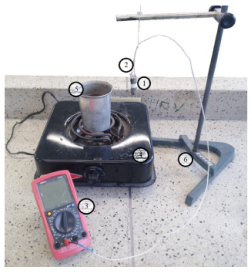
\includegraphics{Montaje.png}
    \caption{Montaje experimental: Ley de enfriamiento.}
    
\end{figure}
\section{Resultados y Análisis}


\section{Conclusiones}


\begin{thebibliography}{15}
   {prof} Evelio, R. J.(2023). Ley de enfriamiento
\end{thebibliography}
\end{document}
